%%%%%%%%%%%%%%%%%%%%%%%%%%%%%%%%%%%%%%%%%%%%%%%%%%%%%%%%%%%%%
%% Prolog
%%%%%%%%%%%%%%%%%%%%%%%%%%%%%%%%%%%%%%%%%%%%%%%%%%%%%%%%%%%%%
\chapter{Aufgabe 5}
\label{sec:aufgabe5}

\subsection*{a)}
Lösen Sie die Aufgaben von Folie 25 (rechte Spalte der Tabelle), 26 (Berechnung Fakultät) und 28 (Anfragen letzter Spiegelpunkt) aus Eck-Prolog.pdf.
\newline

\subsection*{a - Lösung}
\newline

\begin{table}[h]
\centering
\begin{tabular}{@{}lll@{}}
\toprule
List 1              & List 2                                                & Result                                     \\ \midrule
{[}X,Y,Z{]}         & \multicolumn{1}{l|}{{[}john,likes,fish{]}}            & X = john, Y = likes, Z = fish              \\
{[}cat{]}           & \multicolumn{1}{l|}{{[}X|Y{]}}                        & X = cat, Y = {[}{]}                        \\
{[}X,Y|Z{]}         & \multicolumn{1}{l|}{{[}mary,likes,wine{]}}            & X = mary, Y = likes, Z = {[}wine{]}        \\
{[}{[}the,Y{]}|Z{]} & \multicolumn{1}{l|}{{[}{[}X,hare{]},{[}is,here{]}{]}} & X = the, Y = hare, Z = {[}{[}is,here{]}{]} \\
{[}golden|T{]}      & \multicolumn{1}{l|}{{[}golden,norfolk{]}}             & T = {[}norfolk{]}                          \\
{[}white,horse{]}   & \multicolumn{1}{l|}{{[}horse,X{]}}                    & false                                      \\
{[}white|Q{]}       & \multicolumn{1}{l|}{{[}P,horse{]}}                    & P = white, Q = {[}horse{]}                 \\ \bottomrule
\end{tabular}\label{tab:folie25}
\caption{Tabelle}
\vspace{2mm}
\end{table}

\newline
\begin{code}[language=prolog, caption={Fakultät}, label={lst:Aufgabe5a}]
fak(0, 1).
fak(N, F):-
    N > 0,
    N1 is N - 1,
    fak(N1, F1),
    F is N * F1.
\end{code}
\newline
Die Exit-Strategie der Fakultät ist in der Regel \textit{fak(0, 1).} definiert.
Das Prädikat \textit{fak(N, F)} ist die Rekursion, die die Fakultät der nächst kleineren Zahl berechnet und mit der aktuellen Zahl multipliziert.
\newline
\begin{figure}[H]
    \centering
	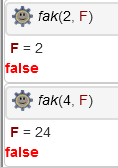
\includegraphics[width=0.3\textwidth]{media/Aufgabe5a_fak}
	\caption{Aufrufe für die Fakultät}
	\label{img:Aufgabe5a_fak}
\end{figure}
\newline

\begin{figure}[H]
    \centering
	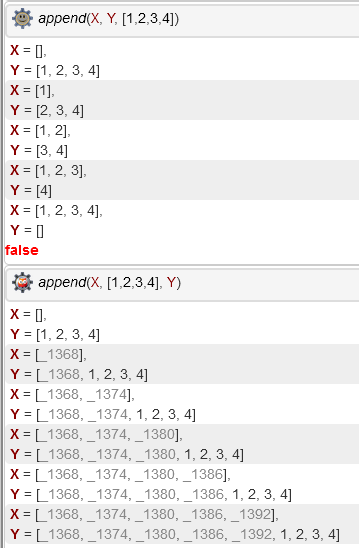
\includegraphics[width=0.5\textwidth]{media/Aufgabe5a_append}
	\caption{Append}
	\label{img:Aufgabe5a_append}
\end{figure}

\newline
Die erste \textit{append} Anfrage liefert alle möglichen Kombinationen von \textit{X} und \textit{Y} zurück, welche zusammen
die Liste \textit{[1, 2, 3, 4]} ergeben.
Wichtig ist dabei, dass die Reihenfolge erhalten bleibt.
Somit ergeben sich \textit{5} mögliche Kombinationen.
\newline
Die zweite \textit{append} Anfrage liefert alle möglichen Kombinationen von \textit{X} und der Liste \textit{[1, 2, 3, 4]} zurück,
welche zusammen die Liste \textit{Y} ergeben.
Somit also unendlich Kombinationen, an denen mindestens die Liste \textit{[1, 2, 3, 4]} anhängt.

\subsection*{b)}
Programmieren Sie ein Prädikat \textbf{sum}, das die Summe einer Liste von Zahlen berechnet.
\textit{Hinweis: Sie müssen Rekursion verwenden.}
\newline

\subsection*{b - Lösung}
\newline
\begin{code}[language=prolog, caption={Sum}, label={lst:Aufgabe5b}]
sum([], 0).
sum([H|T], R) :-
   sum(T, Rest),
   R is H + Rest.
\end{code}
\newline
\begin{figure}[h]
    \centering
	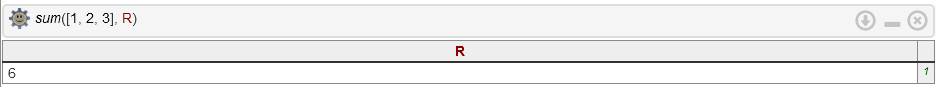
\includegraphics[width=\textwidth]{media/Aufgabe5b_sum}
	\caption{Aufruf von \textbf{sum([1, 2, 3], R)}}
	\label{img:Aufgabe5b_sum}
\end{figure}
\newline

\subsection*{c)}
Sie wollen zu einer Werksbesichtigung von BioNTech in Mainz reisen. Dazu brauchen Sie eine Bahnverbindung. Gegeben sind die folgenden Fakten:

\begin{align*}
  &\textbf{zug(konstanz, 08.39, offenburg, 10.59).}   \\
  &\textbf{zug(konstanz, 08.39, karlsruhe, 11.49).}   \\
  &\textbf{zug(konstanz, 08.53, singen, 09.26).}      \\
  &\textbf{zug(singen, 09.37, stuttgart, 11.32).}     \\
  &\textbf{zug(offenburg, 11.29, mannheim, 12.24).}   \\
  &\textbf{zug(karlsruhe, 12.06, mainz, 13.47).}      \\
  &\textbf{zug(stuttgart, 11.51, mannheim, 12.28).}   \\
  &\textbf{zug(mannheim, 12.39, mainz, 13.18).}       \\
\end{align*}
\newline
Definieren Sie ein Prädikat \textbf{verbindung}, das beschreibt, ob zwischen zwei Städten nach einer gegebenen Abfahrtszeit eine Verbindung inklusive Umsteigen existiert.
\textit{Hinweise: Sie brauchen auch hier Rekursion. Beim Umsteigen muss Abfahrtszeit > Ankunftszeit gelten.}

Ein Abfrage \textbf{verbindung(konstanz, 8.00, mainz, Reiseplan)} soll nacheinander die möglichen Reiseverbindungen nach 8 Uhr in der Listenvariablen \textbf{Reiseplan} liefern.
\newline

\subsection*{c - Lösung}
\newline
\begin{code}[language=prolog, caption={Verbindung}, label={lst:Aufgabe5c}]
zug(konstanz, 08.39, offenburg, 10.59).
zug(konstanz, 08.39, karlsruhe, 11.49).
zug(konstanz, 08.53, singen, 09.26).
zug(singen, 09.37, stuttgart, 11.32).
zug(offenburg, 11.29, mannheim, 12.24).
zug(karlsruhe, 12.06, mainz, 13.47).
zug(stuttgart, 11.51, mannheim, 12.28).
zug(mannheim, 12.39, mainz, 13.18).

verbindung(Start,Uhr,Ziel,Res) :-
    zug(Start,SUhr,Ziel,EndZeit),
    SUhr >= Uhr,
    append([Start,SUhr,Ziel,EndZeit],[],Res)
    ;
    zug(Start,SUhr,Neu,EndZeit),
    SUhr >= Uhr,
    verbindung(Neu,EndZeit,Ziel,L),
    append([Start,SUhr,Neu,EndZeit],L,Res).
\end{code}
\newline
Das \textit{Semikolon (;)} teilt das Prädikat in zwei Fälle auf.
Der erste stellt dabei unsere Exit-Strategie der Rekursion dar.
Hier wird, wenn eine Zugverbindung von \textit{Start} nach \textit{Ziel} existiert, die Liste \textit{Res} mit den entsprechenden
Daten befüllt.
\newline
Wenn keine direkte Verbindung existiert, wird der zweite Fall aufgerufen.
Dabei wird erst die Grundbedingung geprüft, ob ein Zug \textit{Neu} existiert, für den eine Verbindung existiert, bei der
die Abfahrtszeit größer oder gleich der gegebenen Uhrzeit ist.
Anschließend wird rekursiv geprüft, ob eine Folgeverbindung existiert, welche dann ihre Teilstrecke in eine Liste \textit{L} schreibt.
So sammeln sich die Teillisten rekursiv in der Gesamtliste \textit{Res} zusammen.
\newline
\begin{figure}[h]
    \centering
	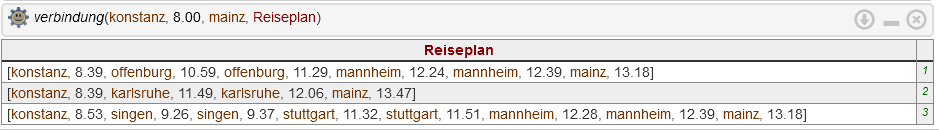
\includegraphics[width=\textwidth]{media/Aufgabe5c_verbindung}
	\caption{Aufruf von \textbf{verbindung(konstanz, 8.00, mainz, Reiseplan)}}
	\label{img:Aufgabe5c_verbindung}
\end{figure}
\newline
